% https://tex.stackexchange.com/a/760767/322482
\documentclass[tikz,border=5pt]{standalone}
\usepackage{tkz-euclide}
\usepackage{fourier}
\begin{document}

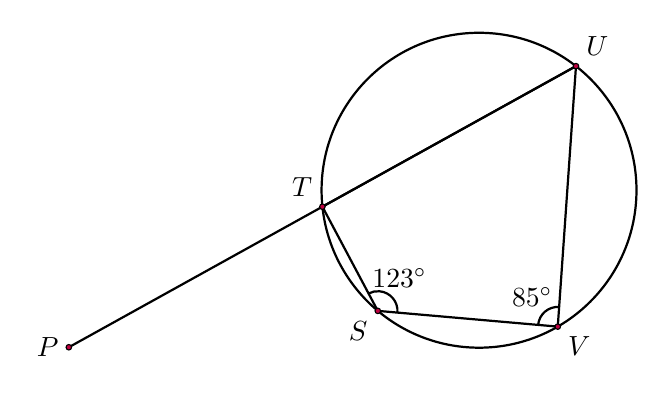
\begin{tikzpicture}
    \tkzSetUpLine[black,thick]
    \tkzDefPoints{0/0/O}
    \foreach \myang/\mylabel in {52/U,-60/V,-130/S,-174/T}{
        \tkzDefPoint(\myang:2){\mylabel}
    }
    \tkzDrawCircle[black,thick](O,U)
    \tkzDrawPolygon(U,V,S,T)
    % \tkzDrawLine[add=0 and 1](U,T)
    \tkzDefPointWith[linear,K=2](U,T)
    \tkzGetPoint{P}
    \tkzDrawSegment(U,P)
    \tkzPicAngle["$123^\circ$",thick,draw,angle eccentricity=2,angle radius=.25cm](V,S,T)
    \tkzPicAngle["$85^\circ$",thick,draw,angle eccentricity=2,angle radius=.25cm](U,V,S)
    \tkzDrawPoints[fill=purple](P,U,V,S,T)
    \tkzLabelPoint[above right](U){$U$}
    \tkzLabelPoint[below right](V){$V$}
    \tkzLabelPoint[below left](S){$S$}
    \tkzLabelPoint[above left](T){$T$}
    \tkzLabelPoint[left](P){$P$}
\end{tikzpicture}

\end{document}